\documentclass[../thesis.tex]{subfiles}

\chapter{Results}\label{results}
This chapter presents the results of the study
which will be used to evaluate
the prototype with respect to whether or not it makes
vocal programming more efficient.


\section{Interview (Part 1)}%
\label{sec:interview_1}

\subsection{Prior Experience}%
\label{sub:prior_experience}
Participants were asked about their level of experience with programming in general, Talon, 
as well as the tools that were the targets for the prototype (Elm and Vim),
see \Vref{tab:experience}.

It should be noted that the amount of time they had been using Talon
does not necessarily correspond with their level of proficiency.
How fast users become proficient with Talon depends on many factors
such as employment status and how much their health allows them to invest time into learning it.
P4 have been using Talon for the shortest amount of time (3 month), but was among the most proficient
out of the six participants.
P3 was the only one that was using Dragon before they started using Talon.

None of the participants had an experience with Elm, although two knew Haskell.
This did not have any effect on the study beyond one participant
being momentarily confused by the result of the \textit{call} command
as they did not know the syntax for function invocation in Elm.

The group had mixed experience levels with Vim.
The less experienced participants would make a few
more mistakes during the test due to forgetting to enter insert mode, 
but it did not impact the study in any significant way.

Five of the six participants had already been programming for many years
and were very familiar with the concepts of parse trees and nodes
in the context of programming languages.
P2 who reported the lowest amount of programming experience
was at least somewhat familiar with the concepts and had no problems
understanding the ideas behind the system.

\begin{table}[htpb]
    \centering
    \begin{tabular}{|c|c|c|c|c}
           \hline 
           & Programming&Talon&Elm&Vim\\
           \hline 
        P1 & 16 years&1 year&Knows Haskell&No Experience\\
        P2 & 1-2 years&1-2 years&No Experience&Little Experience\\
        P3 & 14 years&1 year*&No Experience&No Experience\\
        P4 & 25 years&3 months&No Experience&Very Experienced\\
        P5 & 20 years&1 year&Knows Haskell&Somewhat Experienced\\
        P6 & 25 years&1 year&No Experience&Very Experienced\\
           \hline 
    \end{tabular}
    \caption{Participants Experience}
    \label{tab:experience}
\end{table}


\begin{table}[htpb]
    \centering
    \begin{tabular}{|c|c|c|c|c|}
           \hline 
        & Talon Usage&Speech Engine&Command Set&Platform\\
           \hline 
        P1 &80\%&Conformer&knausj&Linux\\
        P2 &80\%*&Dragon&knausj&Mac\\
        P3 &90\%*&Dragon&knausj&Windows\\
        P4 &60\%&Conformer&knausj*&Mac\\
        P5 &50\%&Conformer&knausj*&Mac\\
        P6 &99\%&Conformer&knausj&Linux\\
           \hline 
    \end{tabular}
    \caption{Participants Setup}
    \label{tab:setup}
\end{table}

\subsection{Issues With Using Talon}%
\label{sub:issues_with_talon}
Before having them try the prototype, participants were asked about what they perceived to be the most significant challenge
with using Talon currently.
The issues mentioned are visualized in \Vref{fig:challenges_cloud}.

The most common issue that is directly related to the task of programming was navigating within a single file.
Participants expressed some frustration with the way they were navigating
code which often involved using line numbers, and iteratively stepping through the words in the line.
This ties into the issue mentioned by P1 of voice control having a significantly slower feedback loop
compared to keyboard and mouse.
Navigating by voice the same way you would with keyboard is very repetitive
and causes more vocal strain, which were major concerns for P2 and P6.
Navigating in this fashion also increases the cognitive load as they must execute more
commands in order to achieve the task.

All participants stated that they are overall slower with voice control 
than they were with keyboard, although they find Talon faster for certain tasks 
that they do often and are familiar with.
The major time loss seems to be misrecognition of dictated text due to
homophones and identifiers often including domain specific words and abbreviations.
Identifiers being misrecognized forces the user to resort to spelling, 
which is repetitive and make the voice control feel low-level and verbose.

\begin{figure}[htpb]
    \centering
    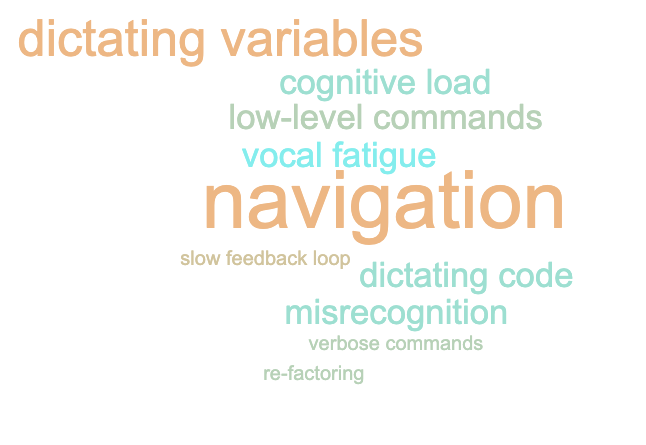
\includegraphics[width=0.8\linewidth]{images/word_cloud.png}
    \caption{Challenges of Talon Users}%
    \label{fig:challenges_cloud}
\end{figure}

\section{Usability Test}%
\label{sec:usability_test}
Participants were given a list of example commands to try to execute
while I observed the response of the system.
The usability test showed that the system worked very well.
Participants were able to navigate and edit code
seamlessly after less than fifteen minutes of usage.
Dictation capabilities were somewhat limited in the current prototype,
but dictation of type signatures worked quite well aside from the issue discussed in \Vref{sub:engine_differences}.

\subsection{How Well Did Participants Understand the System?}%
\label{sub:how_well_did_participants_understand_the_system_}
Participants were able to understand the system very quickly.
Some of the more experienced participants were already familiar with structural editing
and concepts in programming languages, and were able to spot
some of the more subtle features such as when navigating to a string
, it would skip strings within comments.
The less experienced participants did however not have any issues
understanding the concepts once pointed out to them.




\subsection{Engine Differences}%
\label{sub:engine_differences}
Users of \textit{Conformer}, a new model for the \textit{wev2letter} speech engine, ran into an issue when dictating the
\textit{Msg} type.
The system had only been tested with \textit{Dragon} which happened to be able to
recognize ``msg'' as ``message''.
This could have been avoided by adding (msg, message) to the list of overrides,
as was done with \textit{init}.
When generating voice commands for Talon it is important to
test with multiple speech engines to make sure that the system is not relying
on any special features of any particular engine.

\subsection{User Experience Considerations}%
\label{sub:user_experience_considerations}
P6 brought up a potential issue with deleting nodes that are currently off screen.
The execution of the command happens very fast and involves multiple actions
that caused the text on screen to shift.
This can be surprising to new users, but most importantly
it is difficult to verify visually that the command did what it was supposed to do.
With voice control the risk of commands being misrecognized is always present, 
so this must be accounted for by making sure the user can clearly see what's going on.
The participants suggests adding a delay between navigating to, and deleting
a node that is far away.




\section{Interviews (Part 2)}%
\label{sec:interviews_part_2_}

\subsection{General Impressions}%
\label{sub:general_impressions}
All participants reported a positive impression of the prototype.
Several immediately stated that it seems really useful and that they were
very impressed.
P3 describes the system as ``accurate and intuitive'',
and P1 used the phrase ``game changer''.

\subsection{Was the Prototype Intuitive?}%
\label{sub:was_the_prototype_intuitive_}
All participants reported that the prototype expected as they expected
and was overall intuitive.
P1, P3 and P5 did however point out an inconsistency in the Talon grammar
used during the test.
As they noted themselves, this is not really an issue because
the grammar would be part of the user configuration which they would be
able to easily change or rewrite completely themselves.

\subsection{Favorite Features}%
\label{sub:favorite_features}
Participants were asked if they found any future particularly useful.
Five out of six participants mentioned navigating to nodes by their
associated identifier as a standout feature.
P3 was most impressed by the symbol awareness, stating:
``It was very useful that formatting [of identifiers] gets picked up automatically such as with onClick''.
The example they are referring to is the \textit{call {user.functions}} command
which allow them to say ``call on click'' to produce ``onClick''<space>.
P2 also mentioned selecting nodes easily would be very useful
for the kinds of tasks they do often.
P5 mention both structural navigation and editing, but also stated that
``exposing identifiers is the most important feature'' arguing that
this is the part of the system that is the most reusable
and that other people can build upon it in their own scripts.
This sentiment was also expressed by P1.
P6 said that ``everything was better than what I'm currently using''.

\subsection{Requested Features}%
\label{sub:requested_features}
The most requested feature was, as expected, support for more languages and editors
as well as adding awareness of more kinds of syntax nodes.
The fact that the prototype is only aware of symbols within a single file
and cannot perform project wide navigation is a clear limitation, as it was pointed out by several participants.

Being able to move nodes in a single command was mentioned by P2 and P4.
This is a feature that can be implemented user level
and does not require any extensions to the backend.

P6 requested the ability to dictate identifiers containing abbreviations, which was discussed in
\Vref{overrides}.

\subsection{System Relevance}%
\label{sub:system_relevance}
In order to evaluate the systems effectiveness in making vocal programming more efficient,
participants were asked if they feel like the system addresses some of the challenges you have been experiencing with vocal programming.
Four out of six participants immediately answered yes.
P1 reiterates how much of an improvement the navigation is,
and P5 says it makes vocal programming feel more high-level.

P4 is a bit hesitant to say whether or not it directly addresses existing challenges
, but also says that it is still an improvement.
This participant does note that they already have a very advanced solution for navigation
in their editor through a plug-in that have not yet been released.
Some of the features of this system therefore overlap with their solution, but
my solution might be better for global navigation.

P2 answered that for their particular use case, their issues was not
addressed as directly, but they still think it's a useful addition.
The navigational features were again mentioned as being particularly useful.

\subsection{System Interest}%
\label{sub:system_interest}
When asked if they would be interested in using a finished version of the system,
all participants said yes.
Several also noted that the system would not need to be finished,
and they would use it as soon as it supports their languages
and editors.
P2, P4 and P5 expressed interest in contributing to the project
if I was interested in working on it after the thesis is finished.
P3 stated they would like to see the finished thesis.

\section{Assessment of Tools}%
\label{sec:assessment_of_tools}
The main tool used for implementation of this prototype was TreeSitter
, while LSP and Regular Expressions were not used.
TreeSitter proved to be an excellent tool for this task due to its error robustness,
performance, and support for multiple languages.
The Query API enabled a large portion of the backend logic
to be agnostic of the language being analyzed which makes the system
much easier to extend.
The prototype developed for this project shows that TreeSitter can
easily be used to enable high-level syntactic analysis for external systems
such as Talon.



